% Influence of overtaking or lane formation on the success of the model

\begin{figure}[h!]
	\centering
		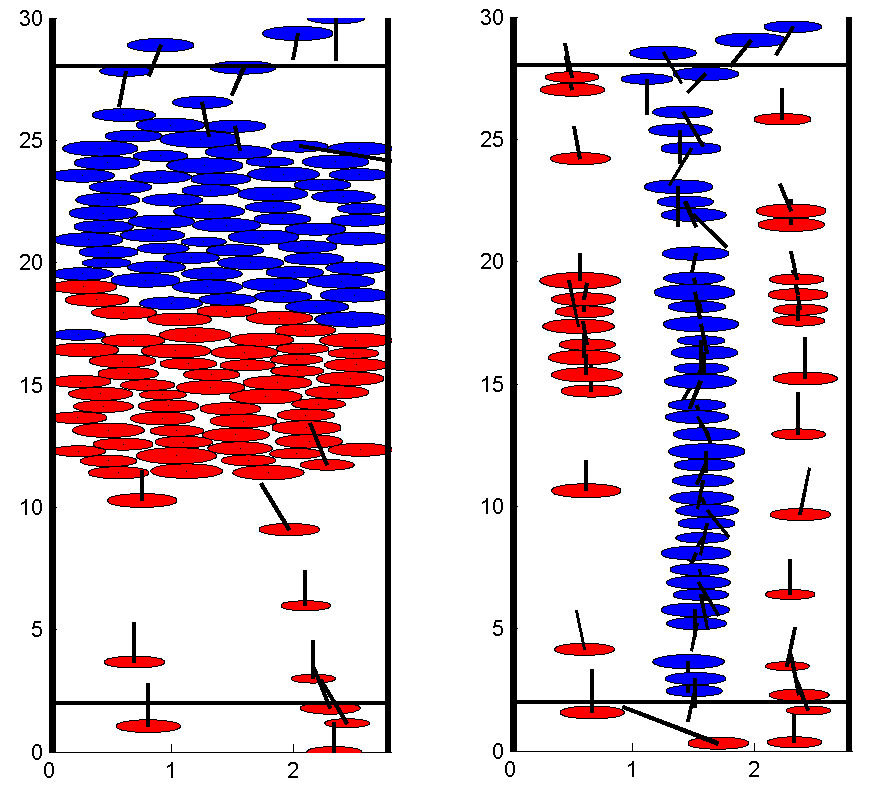
\includegraphics[width=0.8\textwidth]{pictures/ex2picture.png}
	\caption{Exemplary pictures of our simulation after a simulation time of 120 seconds. The left one was run with a \texttt{DISPERSIONFACTOR} of 1 while the right picture has one of 0.1. The jaming to the left and the lane formation to the right can be seen.}
	\label{fig:ex2picture}
\end{figure}

\noi Some examples of how our simulation did look like after a simulation time of 120 second are given in figure \ref{fig:ex2picture}.\\

\noi In figure \ref{fig:AAllInOne} all collected data is consensed into one graph which was visualized in two ways. Another representation of the same data is given in the appendix in figure \ref{fig:ADistanceSeedsFactors} (page \pageref{fig:ADistanceSeedsFactors}). They correlate the average distance covered per agent per iteration step with the simulation time. There were two expectations: As soon as a jam starts to form, this variable should decrease quite fast. Any kind of lane formation should be detectable as most agents will not be able to walk with their maximum speed so the average distance per agent per timestep should be significantly below the mean value given by $\bar{d} = \Delta t \cdot \bar{v}$, the product of \texttt{DELTAT} with \texttt{MEANSPEED}.\\

\begin{figure}[h!]
	\centering
		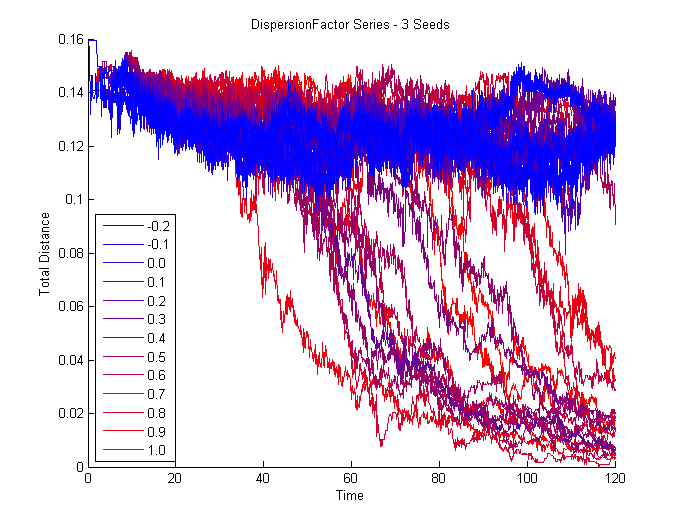
\includegraphics[width=0.49\textwidth]{pictures/AAllInOneColorsBlue.png}
		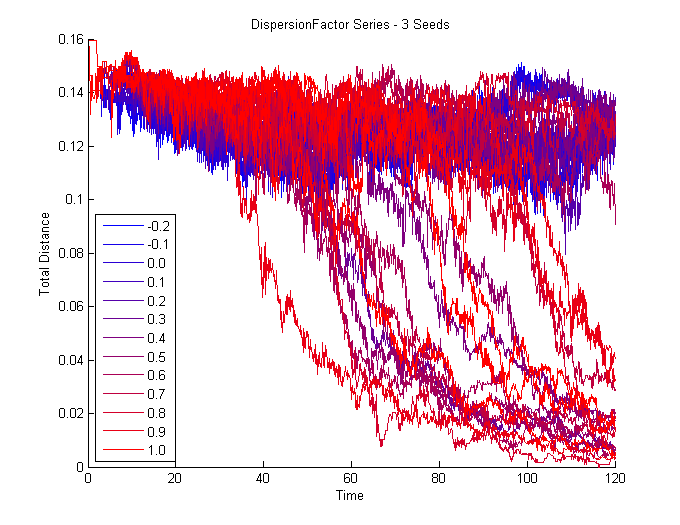
\includegraphics[width=0.49\textwidth]{pictures/AAllInOneColorsRed.png}
	\caption{Graph of the average covered distance per agent present in the simulation per step as a function of time. The more blueish the color is, the stronger was the agents tendency to form lanes while the more reddish the color is, the stronger was the agents tendency to try to overtake slow agents. In the left graph the more blue lines are highlighted while in the right graph the more red lines are highlighted. Although the red lines representing "greedy" agents cope well at the very start, the usually lead to a jam very quickly.}
	\label{fig:AAllInOne}
\end{figure}

\noi Given the two graphs, it is striking that the majority of the simulations represented by reddish lines representing high values of \texttt{DISPERSIONFACTOR} fail during the observed time frame. At rare occasion though the simulation was successful even with a relatively high \texttt{DISPERSIONFACTOR}.\\
On the other side, there was always lane formation for a \texttt{DISPERSIONFACTOR} below 0.4, represented by the more blueish lines which ultimately resulted mostly in successful simulations without jamming.\\
The lane formation can be seen quite clearly in the graphs given in figure \ref{fig:AAllInOne}. The reddish lines try to keep the mean distance at almost all cost, this is visible in the initial height of the reddish lines. In contrast, the blueish lines quickly fall down by about 0.02 meters per agent per iteration step which is a precise indication of lane formation. But in the long run, the best reddish line performed about equally well as most blueish lanes, indicating that in crowded situations like this, cooperation between agents in the form of line formation is not worse in performance as the best egoistic approach, but succeeds way more often.\\

\noi Summing up, it seems that the forced lane formation was a successful way to resolve the problem of jamming. It also highlights the importance of cooperation and the sensitivity of our model towards this parameter.

